%%% template.tex
%%%
%%% This LaTeX source document can be used as the basis for your technical
%%% paper or abstract.

%%% The parameter to the ``documentclass'' command is very important.
%%% - use ``review'' for content submitted for review.
%%% - use ``preprint'' for accepted content you are making available.
%%% - use ``tog'' for technical papers accepted to the TOG journal and
%%%   for presentation at the SIGGRAPH or SIGGRAPH Asia conference.
%%% - use ``conference'' for final content accepted to a sponsored event
%%%   (hint: If you don't know, you should use ``conference.'')

\documentclass[review]{acmsiggraph}
\usepackage{amsmath}
\usepackage{amssymb}
\usepackage{wasysym}
\usepackage[scaled=.92]{helvet}
\usepackage{times}
\usepackage{graphicx}
\usepackage{parskip}
\usepackage{url}
\usepackage[labelfont=bf,textfont=it]{caption}
\usepackage{color}
\usepackage{algorithm}
\usepackage{algorithmic}
\usepackage{enumitem}
\usepackage{authblk}

%----------------------------------------------------------------------------
%----------------------------------------------------------------------------
\definecolor{AdamColor}{rgb}{0,0,0.7}
\definecolor{BenColor}{rgb}{0,0.7,0}
\definecolor{tamarColor}{rgb}{0.8,0,0.8}
\definecolor{JoshColor}{rgb}{0.0,0.7,0.8}
\newcommand{\mycomment}[1]{}
\newcommand{\adam}[1]{{\color{AdamColor} #1}}
\newcommand{\ben}[1]{{\color{BenColor} #1}}
\definecolor{nilsCol}{rgb}{0.85,0.35,0.25}
\newcommand{\Nils}[1]{\textcolor{nilsCol}{#1}}
\newcommand{\tamar}[1]{\textcolor{tamarColor}{#1}}
\newcommand{\josh}[1]{\textcolor{JoshColor}{#1}}
% for final
%\newcommand{\adam}[1]{{#1}}
%\newcommand{\Nils}[1]{{#1}}

%\let\shortcite=\cite
%\newcommand{\shortcite}[1]{\cite{#1}}
\newcommand{\etal}{and colleagues}
\newcommand{\Mueller}{M\"uller~}
\newcommand{\BM}[1]{\B{#1}}
%\newcommand{\B}[1]{\mbox{\boldmath$#1$}}
%\newcommand{\B}[1]{\textbf{\textit{#1}}}
\newcommand{\B}[1]{\mathit{\mathbf{#1}}}
\newcommand{\Per}{\%}
\newcommand{\Unit}[1]{{\mbox{$\,\mathrm{#1}$}}}
\newcommand{\Snit}[1]{{\mbox{\small$\mathrm{#1}$}}}
\newcommand{\Tr}[1]{\mathrm{Tr}\left(#1\right)}
\newcommand{\sign}[1]{\mathrm{sign}\left(#1\right)}
\newcommand{\Hz}{\Unit{Hz}}
\newcommand{\MHz}{\Unit{MHz}}
\newcommand{\GHz}{\Unit{GHz}}
\newcommand{\Sec}{\Unit{sec}}
\newcommand{\SPF}{\Unit{sec/frame}}
\newcommand{\Min}{\Unit{min}}
\newcommand{\Max}{\Unit{max}}
\newcommand{\M}{\Unit{m}}
\newcommand{\Nab}{\B{\nabla}}
\newcommand{\TP}{^\mathsf{T}}

\newcommand{\Dist}{\mbox{dist}}

\newcommand{\figureTopBot}[1]{
  \begin{figure}[!tb]{\sloppy #1}\end{figure}
}

\newcommand{\figureTop}[1]{
  \begin{figure}[!t]{\sloppy #1}\end{figure}
}
 
\newcommand{\figureBot}[1]{
  \begin{figure}[!b]{\sloppy #1}\end{figure}
}

\newcommand{\figureWideTop}[1]{
  \begin{figure*}[!t]{\sloppy #1}\end{figure*}
}

\newcommand{\figureWideBot}[1]{
  \begin{figure*}[!b]{\sloppy #1}\end{figure*}
}

\newcommand{\eqAlgn}{\!\!&\!\!}

\newcommand{\Eref}[1]{Equation~(\ref{#1})}
\newcommand{\Erefs}[2]{Equations~(\ref{#1}) and (\ref{#2})}
\newcommand{\eref}[1]{Equation~(\ref{#1})}
\newcommand{\erefs}[2]{Equations~(\ref{#1}) and (\ref{#2})}
\newcommand{\Sref}[1]{Section~\ref{#1}}
\newcommand{\sref}[1]{Section~\ref{#1}}
\newcommand{\srefs}[2]{Sections~\ref{#1} and~\ref{#2}}
\newcommand{\fref}[1]{Figure~\ref{#1}}
\newcommand{\frefAND}[2]{Figures~\ref{#1} and~\ref{#2}}
\newcommand{\frefs}[2]{Figures~\ref{#1} and~\ref{#2}}
\newcommand{\frefss}[3]{Figures~\ref{#1}, \ref{#2}, and~\ref{#3}}
\newcommand{\frefsss}[4]{Figures~\ref{#1}, \ref{#2}, \ref{#3}, and~\ref{#4}}
\newcommand{\Fref}[1]{Figure~\ref{#1}}
\newcommand{\Frefs}[2]{Figures~\ref{#1} and~\ref{#2}}
\newcommand{\Frefss}[3]{Figures~\ref{#1}, \ref{#2}, and~\ref{#3}}
\newcommand{\Frefsss}[4]{Figures~\ref{#1}, \ref{#2}, \ref{#3}, and~\ref{#4}}
\newcommand{\tref}[1]{Table~\ref{#1}}

\renewcommand{\labelenumi}{\arabic{enumi}.}
\renewcommand{\labelenumii}{\alph{enumii}.}
\renewcommand{\labelenumiii}{\roman{enumiii}.}

\newenvironment{algstep}{%
  \begin{enumerate}%
    \setlength{\itemsep}{0in}%
    \setlength{\partopsep}{0in}%
    \setlength{\topsep}{0in}%
}{\end{enumerate}}

%----------------------------------------------------------------------------
%----------------------------------------------------------------------------

%%% Make the ``BibTeX'' word pretty...

\def\BibTeX{{\rm B\kern-.05em{\sc i\kern-.025em b}\kern-.08em
    T\kern-.1667em\lower.7ex\hbox{E}\kern-.125emX}}

%%% Used by the ``review'' variation; the online ID will be printed on 
%%% every page of the content.

\TOGonlineid{70}

%%% Used by the ``preprint'' variation.

\TOGvolume{0}
\TOGnumber{0}

\title{Clustering and Collision Detection for Clustered Shape Matching}
\author[*]{Ben Jones}
\author[**]{Joshua A. Levine}
\author[***]{Tamar Shinar}
\author[*]{Adam W. Bargteil}
\affil[*]{University of Utah}
\affil[**]{Clemson University}
\affil[***]{University of California, Riverside}
\pdfauthor{}

\keywords{Shape Matching, Ductile Fracture}

\begin{document}

%%% This is the ``teaser'' command, which puts an figure, centered, below 
%%% the title and author information, and above the body of the content.

% \teaser{
%   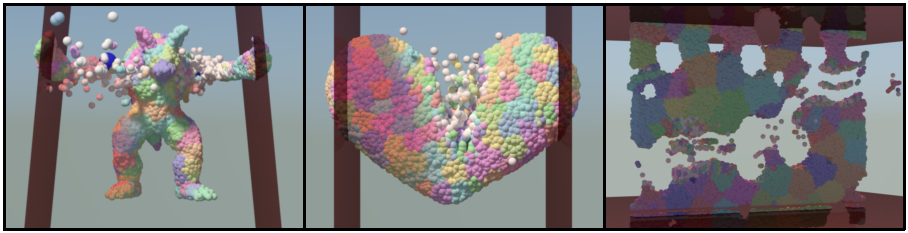
\includegraphics[width=\linewidth]{Figures/teaser}
%   \caption{Left: An armadillo is tortured by being torn apart by the arms while being fired upon by spherical projectiles.  Center: A heartbreaking example.  Right: Tearing a slice of swiss cheese.}
%   \label{fig:teaser}
% }

\maketitle

\begin{abstract}
In this paper, we address clustering and collision detection in the clustered shape matching simulation framework
for deformable bodies.  Our clustering algorithm is ``fuzzy,'' meaning that it gives particles weighted membership in clusters.
These weights are a significant extension to the basic clustered shape matching framework as they
are used to divide particle mass among the clusters.  We explore several weighting schemes
and demonstrate that the choice of weighting scheme gives artists additional control over material behavior.
Furthermore, by design our clustering algorithm yields spherical clusters, which not only results in sparse weight vectors, but
also exceptionally efficient collision geometry.  We further 
enhance this simple collision proxy with halfspaces to allow for even better, yet still simple and computationally efficient, 
collision proxies.  The resulting approach is fast, versatile, and simple to implement.
\end{abstract}

\begin{CRcatlist}
  \CRcat{I.3.7}{Computer Graphics}{Three-Dimensional Graphics and Realism}{Animation};
  \CRcat{I.6.8}{Simulation and Modeling}{Types of Simulation}{Animation}.
\end{CRcatlist}

\keywordlist

%% Required for all content. 

\copyrightspace

\section{Introduction}\label{sec:Introduction}

Introduced a decade ago by \Mueller and
colleagues~\shortcite{Mueller:2005:MDB}, 
{\em shape matching} is a
geometrically motivated technique for animating deformable bodies.
\fref{fig:shapematching} summarizes the method.
The basic approach samples a deformable object with particles, which
determine the degrees of freedom in the object.  Each timestep, a best-fit
rigid transformation of the rest {\em shape} of the object to the 
current configuration of particles is computed and Hookean springs
are used to pull the particles toward the transformed shape.
A powerful extension to this basic approach, also introduced by 
\Mueller and colleagues~\shortcite{Mueller:2005:MDB}, is to break the
object into several overlapping clusters.  We refer to this approach as
{\em clusterd shape matching}.  Having more than one cluster imbues
the object with a richer space of deformation, while overlap keeps
the object from falling apart.
While this approach lacks a well-developed mathematical
underpinning, it has a number of advantages that make it especially
well-suited to interactive graphics applications, such as video games.

In this paper, we address two important aspects of the clustered shape matching framework, namely clustering
and collision detection.
We consider two previously introduced clustering algorithms and introduce a new algorithm tailored to our
specific problem.
Of particular note is that our new clustering algorithm is ``fuzzy,'' 
meaning that particles have weighted membership in clusters.
Weighted membership is a significant extension to the basic clustered shape matching framework and greatly
increases the flexibility of the approach because the weights are used to determine how a particle's
mass is distributed between clusters.
We explore several weighting schemes and demonstrate that the choice of weighting scheme gives 
artists additional control over material behavior.
Furthermore, by design our clustering algorithm forms spherical clusters that, unlike most other fuzzy clustering
techniques, yield sparse and spatially localized weight vectors.

Our clustering method also works well with our approach to collision detection.  The spherical clusters
result in exceptionally convenient collision geometry.  We further 
enhance this simple collision proxy with halfspaces to allow for even better, yet still simple and computationally efficient, 
collision proxies.  The resulting collision detection and handling code is very simple to implement {\em and} computationally efficient.
Combined these extensions significantly enhance the power and versatility of the clustered shape matching framework.

%modeled as volumetric
%point samples.  The geometric distribution of points serves both as a
%descriptor for the body as well as a vehicle for simulating its
%movements.  
%One of their key idea is 
%an extension that uses overlapping clusters of points to model the
%deforming body as opposed to a single point set.

%In this work, we perform further experimentation that develops a
%quantitative evaluation of clustered shape matching.  Specifically, we
%explore five different weighting schemes and three different clustering
%algorithms.  These schemes are aimed to balance computation time with
%cluster distributions while emphasizing results that look good.
%Furthermore, we enrich the cluster shape proxy, adding halfspaces that
%clip the original cluster sphere, enabling clusters to describe fracture
%and other input geometries.  This shape retains the simplicity of
%spherical geometries for collision, but allows for a more accurate
%description of the points that better matches the geometry used
%in simulation.  Together, these contributions allow for heuristics that
%improve the overall quality of clustered shape matching and further
%develop our understanding in absense of a rigorous mathematical
%theory.

\begin{figure*}
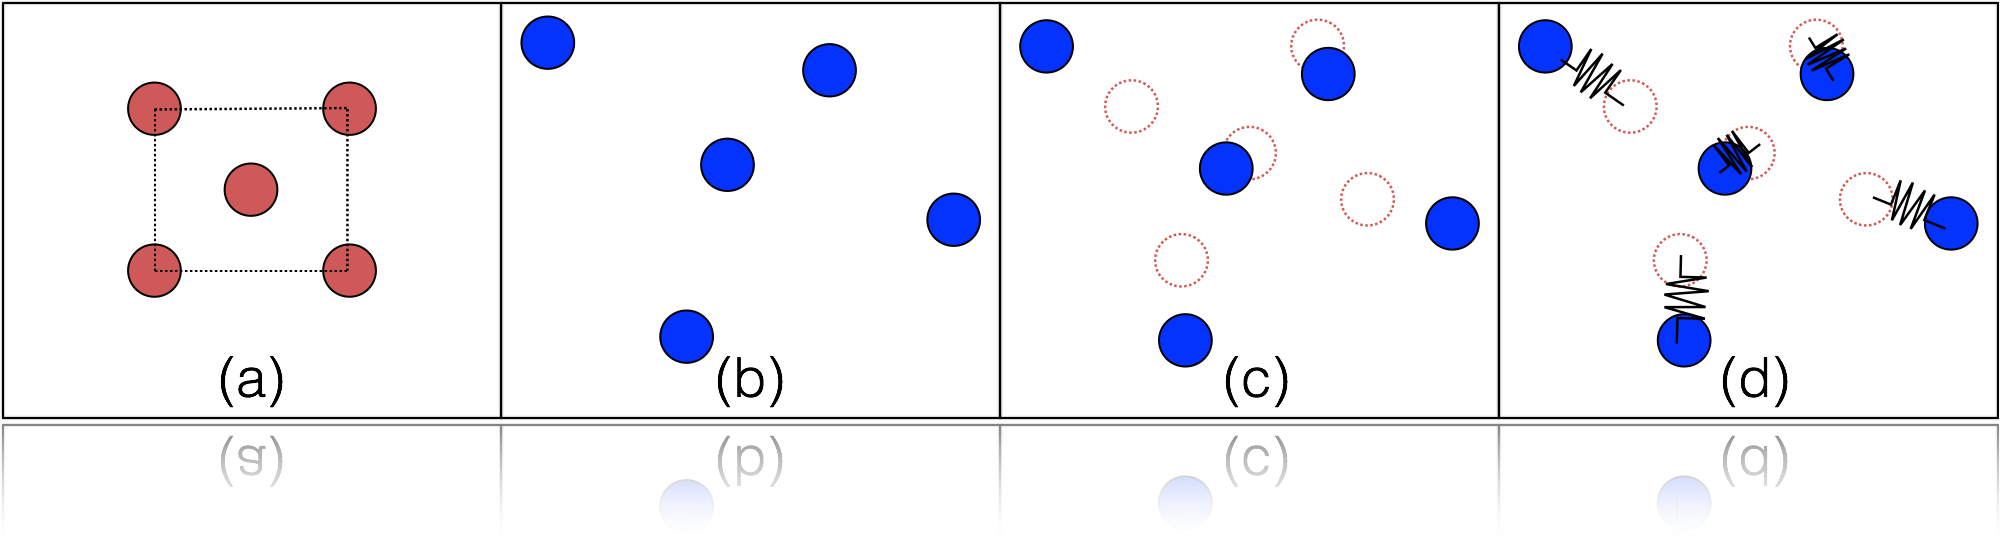
\includegraphics[width=\linewidth]{Figures/shapematching.png}
\caption{Shape Matching Overview: (a) An object (here, a square) is sampled with particles, $p_i$, to get rest positions, $\B{r}_i$.  
(b) As particles are subjected to external forces and constraints, their positions, $\B{x}_i$, are updated in world space.  
(c)  The best-fitting rigid transformation of the particles' rest positions, $\B{r}_i$, 
to their world positions, $\B{x}_i$ is computed.  The dotted red circles are the {\em goal} positions, $\B{g}_i$.  
(d) Hookean springs pull the world positions toward the goal positions.}
\label{fig:shapematching}
\end{figure*}

\section{Related Work}

%Shape matching is a well known approach for simulating deformable
%bodies.  In the original work by \Mueller and colleagues~\shortcite{Mueller:2005:MDB}
%a diverse set of
%physical phenomena are able to be simulated interactively, including
%both rigid and plastic deformations with
%collisions.  Rivers and
%James~\shortcite{Rivers:2007:FFL} introduced a variant to the approach
%based on building a set of hierarchical lattices that define the shape
%matching clusters.  This hierarchy allows for a regular structure that
%improves performance and allows for the inclusion of a simple fracture
%model.  \josh{In a companion work, we develop a ductile fracture
%model~\cite{} -- should we say something like this Josh wonders?}

%Interestingly, while the approach is simple and effective, the research
%community has recently focused more on techniques based on
%position-based
%dynamics~\cite{Mueller:2007:PBD,Bender:2013:PBM,Bender:2014:ASO,Macklin:2014:UPP}
%as opposed to shape matching.  Position-based dynamics boasts many
%advantages, but neither approach is universally best.  For example,
%Bargteil and Jones~\shortcite{Bargteil:2014:SLF} added strain-limiting
%into clustered shape matching and in doing so discovered several
%advantages of shape matching over position-based dynamics.  Most
%significantly, shape matching respects Newton's laws of motion.
%Furthermore, they also suggest that there is a dramatic effect to the
%choice of clustering, motivating this work to explicitly study the
%relationship between clusters and output quality.

The geometrically motivated shape matching approach was introduced by \Mueller and 
colleagues~\shortcite{Mueller:2005:MDB}, who demonstrated impressive results and 
described the key advantages of the approach: efficiency, stability, and controllability.
Given these advantages, shape matching is especially appealing in interactive animation contexts such as
video games.  The authors also introduced several extensions including linear and quadratic deformations 
(in addition to rigid deformations), cluster-based deformation, and plasticity.  
%
Two years later, Rivers and James~\shortcite{Rivers:2007:FFL} introduced lattice-based shape matching,
which used a set of hierarchical lattices to define the shape matching clusters.  They took advantage
of the regular structure of the lattices to achieve extremely high performance.  

Despite impressive results and substantial promise,
the shape matching framework has been largely disregarded by the research community in favor of position-based
dynamics~\cite{Mueller:2007:PBD,Bender:2013:PBM,Bender:2014:ASO,Macklin:2014:UPP}.  One notable exception is
the work of Bargteil and Jones~\shortcite{Bargteil:2014:SLF}, which incorporated strain-limiting into clustered shape matching
and pointed out several advantages of shape matching over position-based dynamics.  Most significantly, shape matching respects Newton's 
laws of motion.

Clustering is well-studied in the machine learning literature and many techniques, such as $k$-means, have become standard tools in computer graphics.  
A complete survey of this literature is beyond the scope of this short paper, but for the sort of ``fuzzy'' clustering we propose in this paper,
we recommend the survey by Nock and Nielsen~\shortcite{Nock:2006:OWC}.  Similarly, collision detection is well-studied in the 
computer graphics and robotics literature.  For a survey of real-time techniques we recommend the text by Ericson~\shortcite{Ericson:2004:RCD}.

\section{Methods}
For completeness and readability, we first briefly review the shape matching approach of \Mueller and colleagues~\shortcite{Mueller:2005:MDB}.  \fref{fig:shapematching} summarizes the approach.  
\subsection{Shape Matching}
\label{sec:ShapeMatching}
In the shape matching framework
objects are discretized into a set of particles, $p_i\in\mathcal{P}$, with masses, $m_i$, and rest positions, $\B{r}_i$, 
that follow a path, $\B{x}_i(t)$, in world space through time.
Shape matching takes its name from the fact that, each frame, we match the rest shape to 
the deformed shape by finding
the least-squares best-fit rigid transformation from the rest pose
to the current deformed pose by
solving for the rotation matrix, $\B{R}$, and translation
vector, $\B{x}_{cm}-\B{r}_{cm}$, that minimizes
\begin{equation}
\label{eq:sm}
\sum_i m_i \| \B{R}\left(\B{r}_i - \B{r}_{cm}\right)-\left(\B{x}_i-\B{x}_{cm}\right)\|^2.
\end{equation}
The best translation is given by the center of mass in the rest and world space.
Computing the rotation, $\B{R}$, is more involved.  
We first compute the least-squares best-fit linear deformation gradient, $\B{F}$.
Specifically, we seek the $\B{F}$ that minimizes
\begin{equation}
\sum_i m_i \| \B{F}\left(\B{r}_i - \B{r}_{cm}\right)-\left(\B{x}_i-\B{x}_{cm}\right)\|^2.
\end{equation}
Setting the derivative with respect to $\B{F}$ to $0$ and re-arranging terms we arrive at
\begin{equation}
\label{eq:defgrad}
\B{F} = \left(\sum_i m_i \B{O}(\B{x}_i,\B{r}_i)\right)\left(\sum_im_i\B{O}(\B{r}_i,\B{r}_i)\right)^{-1} = \B{A}_{xr}\B{A}_{rr}^{-1},
\end{equation}
where $\B{O}(\cdot,\cdot)$ is the outer product matrix
\begin{equation}
\B{O}(\B{a}_i,\B{b}_i) = \left(\B{a}_i-\B{a}_{cm}\right)\left(\B{b}_{i}-\B{b}_{cm}\right)^T,
\end{equation}
and $\B{A}_{**}$ is a convenient shorthand.
%\begin{align}
%\B{F} = &\left(\sum_i m_i\left(\B{x}_{i}-\B{x}_{cm}\right)\left(\B{r}_{i}-\B{r}_{cm}\right)^T\right)\notag\\
%&\left(\sum_i m_i\left(\B{r}_{i}-\B{r}_{cm}\right)\left(\B{r}_{i}-\B{r}_{cm}\right)^T\right)^{-1},
%\end{align}
%and $m_i$ is the mass of $p_i$. 
We then compute $\B{R}$ using the polar decomposition,
\begin{equation}
\label{eq:decomp}
\B{F} = \B{R}\B{S} = \left(\B{UV}^T\right)\left(\B{V\Sigma V}^T\right)
\end{equation}
where $\B{S}=\B{V\Sigma V}^T$ is a symmetric matrix and $\B{U\Sigma V}^T$ is the singular value decomposition (SVD) of $\B{F}$.
While several researchers (e.g.~\cite{Rivers:2007:FFL}) have pointed out that polar decompositions can be computed faster than the SVD,
especially when warm started, the SVD requires a negligible portion of our computation time and, in our experiments, 
the optimized SVD in the Eigen library was faster than our implementations of polar decompositions.  Furthermore, the SVD is more robust in
the presence of degeneracies or inversions.
We also note that we compute the polar decomposition of $\B{F}$, not
the left matrix ($\B{A}_{xr}$)
%($\sum_im_i\B{O}(\B{x}_i,\B{r}_i)$) 
as done by \Mueller and colleagues~\shortcite{Mueller:2005:MDB}.  This modification
is particularly important if the distribution of mass in the cluster is non-uniform and $\B{F}$ is not a pure rotation.

Given $\B{R}$ and $\B{x}_{cm}-\B{r}_{cm}$, we define goal positions, $\B{g}_i$, as
\begin{equation}
\B{g}_i = \B{R}\left(\B{r}_i-\B{r}_{cm}\right)+\B{x}_{cm}.
\end{equation}
Hookean springs are then used to define forces that move the particles toward the goal positions.

\subsection{Clustered Shape Matching}
Handling multiple clusters is straightforward.  When computing a particle's contribution to 
cluster quantities, we must divide the particle's mass among its clusters.  To do 
so we introduce a weight $w_{i,c}$ for particle $p_i$ in cluster $c\in\mathcal{C}$ that describes how much of
$p_i$'s mass is contributed to cluster $c$.  These weights enter into equations \eqref{eq:sm}-\eqref{eq:defgrad} by multiplying
the particle's mass.  As an example, the center of mass of cluster $c$, $\B{x}_{cm,c} = \B{x}_{c}$ (dropping the $_{cm}$ for clarity), is
\begin{equation}
\label{eq:com}
\B{x}_{c} = \frac{\sum_{p_i\in\mathcal{P}_c}(m_iw_{i,c})~\B{x_i}}{\sum_{p_i\in\mathcal{P}_c}(m_iw_{i,c})}% = \frac{\sum_{p_i\in\mathcal{P}_c}(m_i/n_i) \B{x_i}}{\sum_{p_i\in\mathcal{P}_c}(m_i/n_i)},
\end{equation}
where $\mathcal{P}_c$ is the set of particles in cluster $c$.
We experimented with five weighting schemes in our implementation.  The first, and simplest, weighting
scheme divides the particles mass evenly among the $n_i$ clusters it belongs to, $w_{i,c} = 1/n_i$.
%divide the particle's mass by the number of clusters it belongs to,
%essentially replacing $m_i$ with $m_i/n_i$ in equations \eqref{eq:sm}-\eqref{eq:defgrad} 
%and when computing cluster mass and center of mass.
This scheme correspnds to the ``box'' kernel, or constant weights,
\begin{equation}
\label{eq:box}
\mathrm{box}(\B{x}_i, \B{x}_{c}, h) = 1.
\end{equation}
Second is the well-known $\mathrm{poly6}(\cdot)$ kernel~\cite{Mueller:2003:PFS},
\begin{equation}
\label{eq:poly6}
\mathrm{poly6}(\B{x}_i, \B{x}_{c}, h) = \frac{315}{64\pi h^9}\left(h^2-\|\B{x}_i-\B{x}_{c}\|^2\right)^3,
\end{equation}
where $h$ is the kernel width.
Third is a blend of the $\mathrm{box}$ and $\mathrm{poly6}$ kernels
\begin{equation}
\label{blend}
\mathrm{blend}(\B{x}_i, \B{x}_{c}, h) = \beta + \mathrm{poly6}(\B{x}_i, \B{x}_{c}, h),
\end{equation}
where $\beta$ is a blend parameter.
Fourth is a simple inverse distance squared kernel,
\begin{equation}
\label{eq:invdistancesquared}
\mathrm{invsq}(\B{x}_i, \B{x}_{c}, h) = \frac{1}{\|\B{x}_i-\B{x}_{c}\|^2+\epsilon},
\end{equation}
where $\epsilon$ prevents dividing by zero (we use $\epsilon = 0.0001$).
Fifth is the fuzzy $c$-means weighting function~\cite{Dunn:1973:AFR,Bezdek:1981:PRF},
\begin{equation}
\label{eq:fuzzycmeans}
\displaystyle \mathrm{fcm}(\B{x}_i, \B{x}_{c}, h) = \dfrac{1}{\displaystyle \sum_{d\in\mathcal{C}}\left(\dfrac{\|x_i - x_{c}\|}{\|x_i-x_{d}\|}\right)^{\tfrac{2}{m-1}}},
\end{equation}
where $m$ is a user-specified parameter greater than one.
Note that $\mathrm{fcm}$ is the only weighting function where the weight in one cluster depends on the positions of other cluster centers,
which significantly complicates computation.

To ensure that the total mass of the clusters equals the total mass of the particles, for all kernels we normalize our weights to a partition of unity,
\begin{equation}
\label{eq:weights}
w_{i,c} = \frac{\mathrm{kernel}(\B{x}_i, \B{x}_{c}, h)}{\sum_{d\in\mathcal{C}}\mathrm{kernel}(\B{x}_i, \B{x}_{d}, h)}
\end{equation}
As discussed in~\sref{sec:results} the choice of kernel can have significant impact on the results; while we selected
$\mathrm{invsq}$ as our default, our implementation makes it easy to switch between kernels to satisfy artistic goals.

%We also essentially replace $m_i$ with $w_{i,c}m_i$ in equations \eqref{eq:sm}-\eqref{eq:defgrad} 
As noted above, these weights show up in many of our calculations.  As another example,
when computing the goal position, $\B{g}_i$, for a particle we perform a weighted
average of the goal positions given by each cluster it is a part of.  That is,
\begin{equation}
\B{g}_i = \sum_c w_{i,c}~\B{g}_{i,c},
\end{equation}
where $\B{g}_{i,c}$ is the goal position for particle $p_i$ in cluster $c$.

\paragraph{Strain Limiting}
To maintain stability we adopt the strain limiting approach advocated by Bargteil and Jones~\shortcite{Bargteil:2014:SLF}.

\subsection{Clustering}
In our context, there are several desirable properities for a clustering algorithm.  Of utmost importance is that the clusters overlap, 
otherwise the simulated object will fall apart.  The clusters must also include all the particles, preferably with a modest number of clusters.  
Finally, if the clusters are well-approximated by spheres, collision handling becomes far simpler.  While clustering is
very well-studied in machine learning, these properties are unique to our problem and we are not aware of any algorithm tailored to these
constraints.  

In our implementation we experimented with three clustering algorithms.  The first algorithm, $\mathrm{random}$,
borrowed from Bargteil and Jones~\shortcite{Bargteil:2014:SLF}, is a simple randomized scheme that iteratively
chooses a random particle that is not a member of any cluster,
uses its location as the center of a new cluster, and adds all particles within a user-specified distance to the cluster.  
The algorithm terminates when all particles are a member of at least one cluster.  Weights, cluster center of mass, etc.\ are
determined after the algorithm terminates.  The user specifies the {\em neighborhood radius}--- 
maximum distance, $d$, from the cluster center to particles
included into the cluster; this $d$ is then used in a spherical range query to determine cluster membership.
Note that in this algorithm, the user has no direct control over the number of clusters, $|\mathcal{C}|$.

The second algorithm, $\mathrm{kmeans}$, uses $k$-means to determine cluster centers; given $k = |\mathcal{C}|$ 
random seed locations for clusters, this two-step algorithm iteratively
\begin{enumerate}
\item updates cluster membership for each particle by choosing the nearest cluster center;
\item updates cluster centers to be the center of mass of the particles in the cluster.
\end{enumerate}
Convergence is achieved when cluster membership is no longer changing.  
After the $k$-means algorithm terminates overlapping clusters are computed by including
all particles within a user-specified distance, $d$, of the computed cluster centers.  
Finally, membership weights, cluster center of mass, etc.\ are computed.

Our final algorithm, $\mathrm{ours}$, more closely resembles {\em fuzzy $c$-means}~\cite{Dunn:1973:AFR,Bezdek:1981:PRF}, 
but explicitly seeks greater sparsity in the membership weights by forcing
weights for particles far from a cluster center to zero.  As in the previous algorithm, we choose initial cluster centers using $k$-means.
However, we then perform an additional two-step iterative optimization:
\begin{enumerate}
\item update cluster membership {\em and weights};
\item update cluster centers to be the {\em weighted} center of mass of the particles in the cluster.
\end{enumerate}
Instead of computing the nearest cluster center for each particle as in $k$-means, our algorithm includes all particles within a given distance, 
$d$, using a standard spherical range query, which is accelerated with a grid data structure.  Computing the weights 
(\eref{eq:weights}) requires evaluating the above 
kernels for each particle in each cluster and keeping a running sum of the weights for each particle.  Updating the cluster centers simply requires 
computing~\eref{eq:com} for each cluster using the weights computed in the previous step.  To faciliate satisfying the first requirement that 
all particles belong to at least one cluster, we add any particles that are not within the neighborhood radius, $d$, of 
any cluster center to the nearest cluster 
(in a similar manner to the $k$-means algorithm).  Any such particles immediately signal that the algorithm has not converged.  Otherwise,
we declare convergence if cluster membership remains the same for two iterations and the cluster centers have not moved more than $0.1\%$ of the neighborhood radius.   
If the algorithm
does not converge within a limited number of iterations we increase the number of clusters, $|\mathcal{C}|$, and/or the neighborhood radius, $d$, until convergence is achieved.

Compared to $k$-means our algorithm has the advantage of including the fact that clusters should overlap in the optimization itself, which leads to slower convergence, but
also to a clustering that is better suited to our needs.

\subsection{Collision Detection}
We first describe the simple and efficient collision proxy geometry we use for clusters and then describe
our collision detection and handling algorithm.

\paragraph{Collision Geometry}
Because we explicitly include the distance constraint during clustering, the resulting clusters are generally well approximated
by spheres.  However, for some input geometry, such as a thin sheet, this approximation is less than ideal.  Consequently,
we enhance our collision proxy by adding planes.  Specifically, our geometric representation of the collision proxy
is the intersection of a sphere with a set of half-spaces.

The radius of the sphere is given by the user-specified neighborhood radius, $d$.  The center of the sphere is chosen as the 
geometric center of the range query used during clustering---the randomly chosen seed particles for $\mathrm{random}$ algorithm;
the cluster centers given by $k$-means in the $\mathrm{kmeans}$ algorithm; or the cluster centers given by $\mathrm{ours}$.
Note that with $\mathrm{random}$ and $\mathrm{kmeans}$ the algorithmic cluster centers and the physical cluster center of mass will
generally not be the same point.  One advantage of our algorithm is that, because the weighted center of mass is computed during
the optimization, the algorithm's output is the physical center of mass.

As mentioned above we intersect these sphere with half-spaces.  During initialization, after computing the clusters, we examine the 
Eigenvectors, $\B{V}_i$, of the scatter matrix, $\B{A}_{rr}$.  These Eigenvectors give the principal directions that describe the distribution
of particles in the cluster.  We compute the planes normal to these Eigenvectors that bound the particles in the cluster.  Specifically,
for each Eigenvector we compute the dot product with each particle in the cluster, keeping track of the 
minimum and maximum values, yeilding six plane equations of the form
\begin{equation}
\phi(\B{x}) = \B{V}_i\cdot\B{x} + a_j = 0.
\end{equation}
We adopt the convention that points for which $\phi(\cdot)<0$ lie {\em inside} the halfspace.  If a plane lies within a user-specified
distance of the center of the sphere---that is it cuts off a significant portion of the collision volume---we add it to the collision
geometry.  This geometric representation is stored in the rest space of the objcet.  More planes can be added at runtime by projecting
them from world space to rest space using $\B{F}^{-1}$.

For each cluster we also store, in world space, the maximum distance from the center of mass to a member particle, yielding simple
collision proxy in world space.

\paragraph{Collision Detection and Handling}
During runtime, we check for collision between every pair of clusters, $c_1$ and $c_2$.  We explicitly prohibit collisions between
any two clusters that ``overlap,'' or have a particle in common.  To facilitate quickly culling these collisions
we compute cluster overlap maps; each cluster stores
a list of clusters that it cannot collide with.  Computing the overlap maps is somewhat involved; for each particle,
we inform every pair of clusters in the particle's membership list that there is an overlap.
Luckily, these maps can be computed once during initialization if the clusters remain constant.

If two clusters do not have a membership overlap, we next check whether their world space sphere proxies overlap.  If not, 
there is no collision and we continue to the next pair of clusters.  If so, we consider each particle, $p_i$, in the
first cluster, $c_1$.  We first check whether the particle is inside the world space sphere proxy of the second cluster, $c_2$.  If not, 
we continue to the next particle.  If so, we transform the particle's world position into the second cluster's rest space,
Specifically, we compute
\begin{equation}
\B{x}_i^\prime = \B{r}_{c_2} + \B{F}_{c_2}^{-1}\left(\B{x}_i - \B{x}_{c_2}\right)
\end{equation}
We then project $\B{x}^\prime$ onto our simple collision
geometry by taking the minimum of all projections onto the sphere and half-space components.  If the particle lies outside the
sphere or any of the halfspaces, we simply continue to the next particle.  Otherwise, we transform the projected point, $\B{y}_i^\prime$,
to world space to get $\B{y}_i$.  Finally we move the particle toward $\B{y}$.  
Specifically, we update $\B{x}_i$ as
\begin{equation}
\B{x}_i = \B{x}_i + \gamma\left(\B{y}_i-\B{x}_i\right).
\end{equation}
With $\gamma=1$ the collision should be completely resolved.  In complicated collision scenarios, with multiple constraints on any given
particle, choosing $\gamma=1$ can be problematic, so we allow the user to specify the value.

\section{Results and Discussion}
\label{sec:results}

Artists must specify two parameters for our clustering algorithm: the neighbor radius, $d$, and the desired number of clusters, 
$|\mathcal{C}|$.  Additionally, artists may choose between all three of our clustering algorithms ($\mathrm{random}$, $\mathrm{kmeans}$,
and $\mathrm{ours}$) and between all five weighting functions ($\mathrm{box}$, $\mathrm{poly6}$, $\mathrm{blend}$, $\mathrm{invsq}$, 
$\mathrm{fcm}$). The accompanying video includes a variety of examples that explore the effects of these choices with a simple animation
of a cube that is stretched by a factor of 2 in the x-direction and released.
In the first set of examples we show the effect of increasing the number of clusters, $|\mathcal{C}|$, from 1 to 50, while choosing the
minimal neighbor radius that allows convergence.  All these examples use $\mathrm{ours}$ algorithm and the $\mathrm{invsq}$ kernel.
These examples clearly show how more clusters "soften" up the object.  
However, since the neighborRadius is minimal in some sense, there are still fairly sharp boundaries between the clusters.
To illustrate the effect of the neighbor radius, $d$, we fix the number of clusters, $|\mathcal{C}|$, at 10 and increase $d$ from
the minimal value needed for convergence.  With a minimal radius, there are sharp boundaries between the objects.  With a larger
radius the result is smoother.  Using an even larger radius is akin to using fewer clusters.  Thus, there is a complex interaction
between these two parameters.  One approach to authoring would be to first choose the number of clusters and then increase the neighbor
radius from the minimal value until a desired smoothness is acheived.  Automatically tuning the neighbor radius would be an interesting
area for future work.

We also show examples with the different algorithms and different kernels for cluster sizes of 10 and 50.  \adam{It would be nice to say 
something intelligent here.}

Finally, we have a more practical example of a sphere colliding with a thin sheet.  This example demonstrates our approach
to collisions.  Many of the clusters in the thin sheet include the automatically determined halfspaces demonstrating the efficacy
of this approach.  On a typical laptop this example ran at 55 frames per second with rendering, 161 frames per second without rendering.

In conclusion we have significantly extended the clustered shape matching framework for animating deformable bodies by introducing
a new ``fuzzy'' clustering algorithm that produces a highly flexible weight distribution for each particle
and also leads to a simple collision proxy that we enhance with half-spaces.  These approaches will certainly improve the
power and versatility of the clustered shape matching framework.

\mycomment{\begin{table*}
\begin{center}
\caption{Timing results in ms per frame taken on a Macbook Pro with a 2.4Ghz Intel i5 processor.}
\label{table:timing}
\begin{tabular}{|l|l|l|l|l|l|}
\hline
example & \# particles & dynamics & plasticity & fracture & total\\
\hline
armadillo & 20115 & 16  & $<$ 1 & $<$ 1 & 24\\
twisted bar & 5317 & 7 & $<$ 1  & 0 & 7\\
twisted bar with fracture & 5317 & 7  & $<$ 1 & $<$ 1 & 9 \\
projectile & 5325 & 20 & $<$ 1 & $<$ 1 & 29\\
broken heart & 20132 & 22 & $<$ 1 & $<$1 & 31\\
swiss cheese & 25032 & 27 & $<$ 1 & $<$1 & 39 \\
\hline
\end{tabular}
\end{center}
\end{table*}

\paragraph{Limitations and Future Work}

Our blue-noise sampling and $k$-means clustering improve upon the regular grids and
randomized clusters of Bargteil and Jones~\shortcite{Bargteil:2014:SLF} and are effective for our purposes,
but better approaches certainly exist.  In particular, it would be interesting to explore adaptive sampling
so that computational resources can be focused on interesting areas of the object.  
Changing the sampling over time as done by Pauly and colleagues~\shortcite{Pauly:2005:MAO}
is also a promising avenue for future work, which may help address the geometric limitations discussed above.
It would also be interesting
to consider adaptive and hierarchical clustering techniques; the hierarchical lattices of Rivers and James~\cite{Rivers:2007:FFL}
clearly improved performance and artistic directability.  

The biggest limitation of our approach is a lack of theoretical underpinnings for the clustered shape matching
framework; we do not yet have any mathematical tools to analyze the approach.  We do not really understand
how the method behaves as particle counts or timesteps decrease or as the cluster size or number of clusters change.
This limitation does not mean the approach is not useful.  After all, the finite element method was in use
for decades before a mathematical framework was developed to analyze its properties.  In a similar way,
we believe the clustered shape-matching framework will prove extremely useful in practice while
researchers develop mathematical tools for analysis. 

\paragraph{Conclusion} 
One of the primary advantages of the clustered shape matching approach is that the number of degrees of freedom
is much larger then the number of ``integration units''---clusters in this case.  The opposite is true of finite element
methods with unstructured meshes where the number of tetrahedra is often considerably larger than the number of vertices.  
For graphical applications visual detail, which correlates with the number of degrees of freedom, is of paramount importance
and computation, which correlates with ``integration units,'' is often limited.  
For these reasons, the clustered shape matching framework is extremely appealing for computer animation, 
especially interactive animation.  The utility and versatility of this framework is greatly improved by our extensions 
to clustering and collision handling.
}



\section*{Acknowledgements}
Removed for anonymous review.

\bibliographystyle{acmsiggraph}
\bibliography{csm}
\end{document}
